\subsection{Verbesserungsvorschläge Trello}
\FloatBarrier
\begin{figure}[h]
    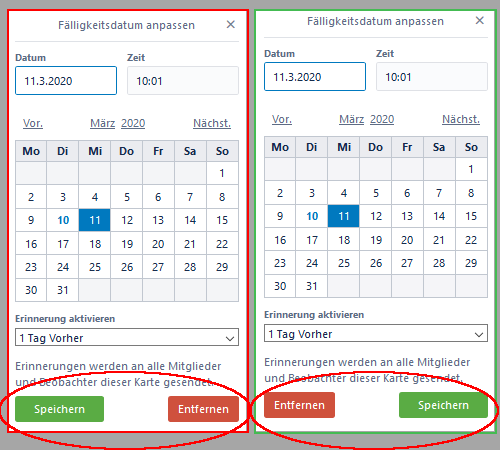
\includegraphics[width=0.5\textwidth]{images/Verbesserungsvorschlaege/1 TrelloDatepicker.PNG}
    \centering
    \caption{Problemgrad 1: Einhaltung des Standards der Leserichtung bei der Platzierung des 'Speichern'-Buttons (Problem Nr. 2, rechts die überarbeitete Version mit dem Button auf der rechten Seite)}
    \label{fig:datepicker}
\end{figure}

\begin{figure}[h]
    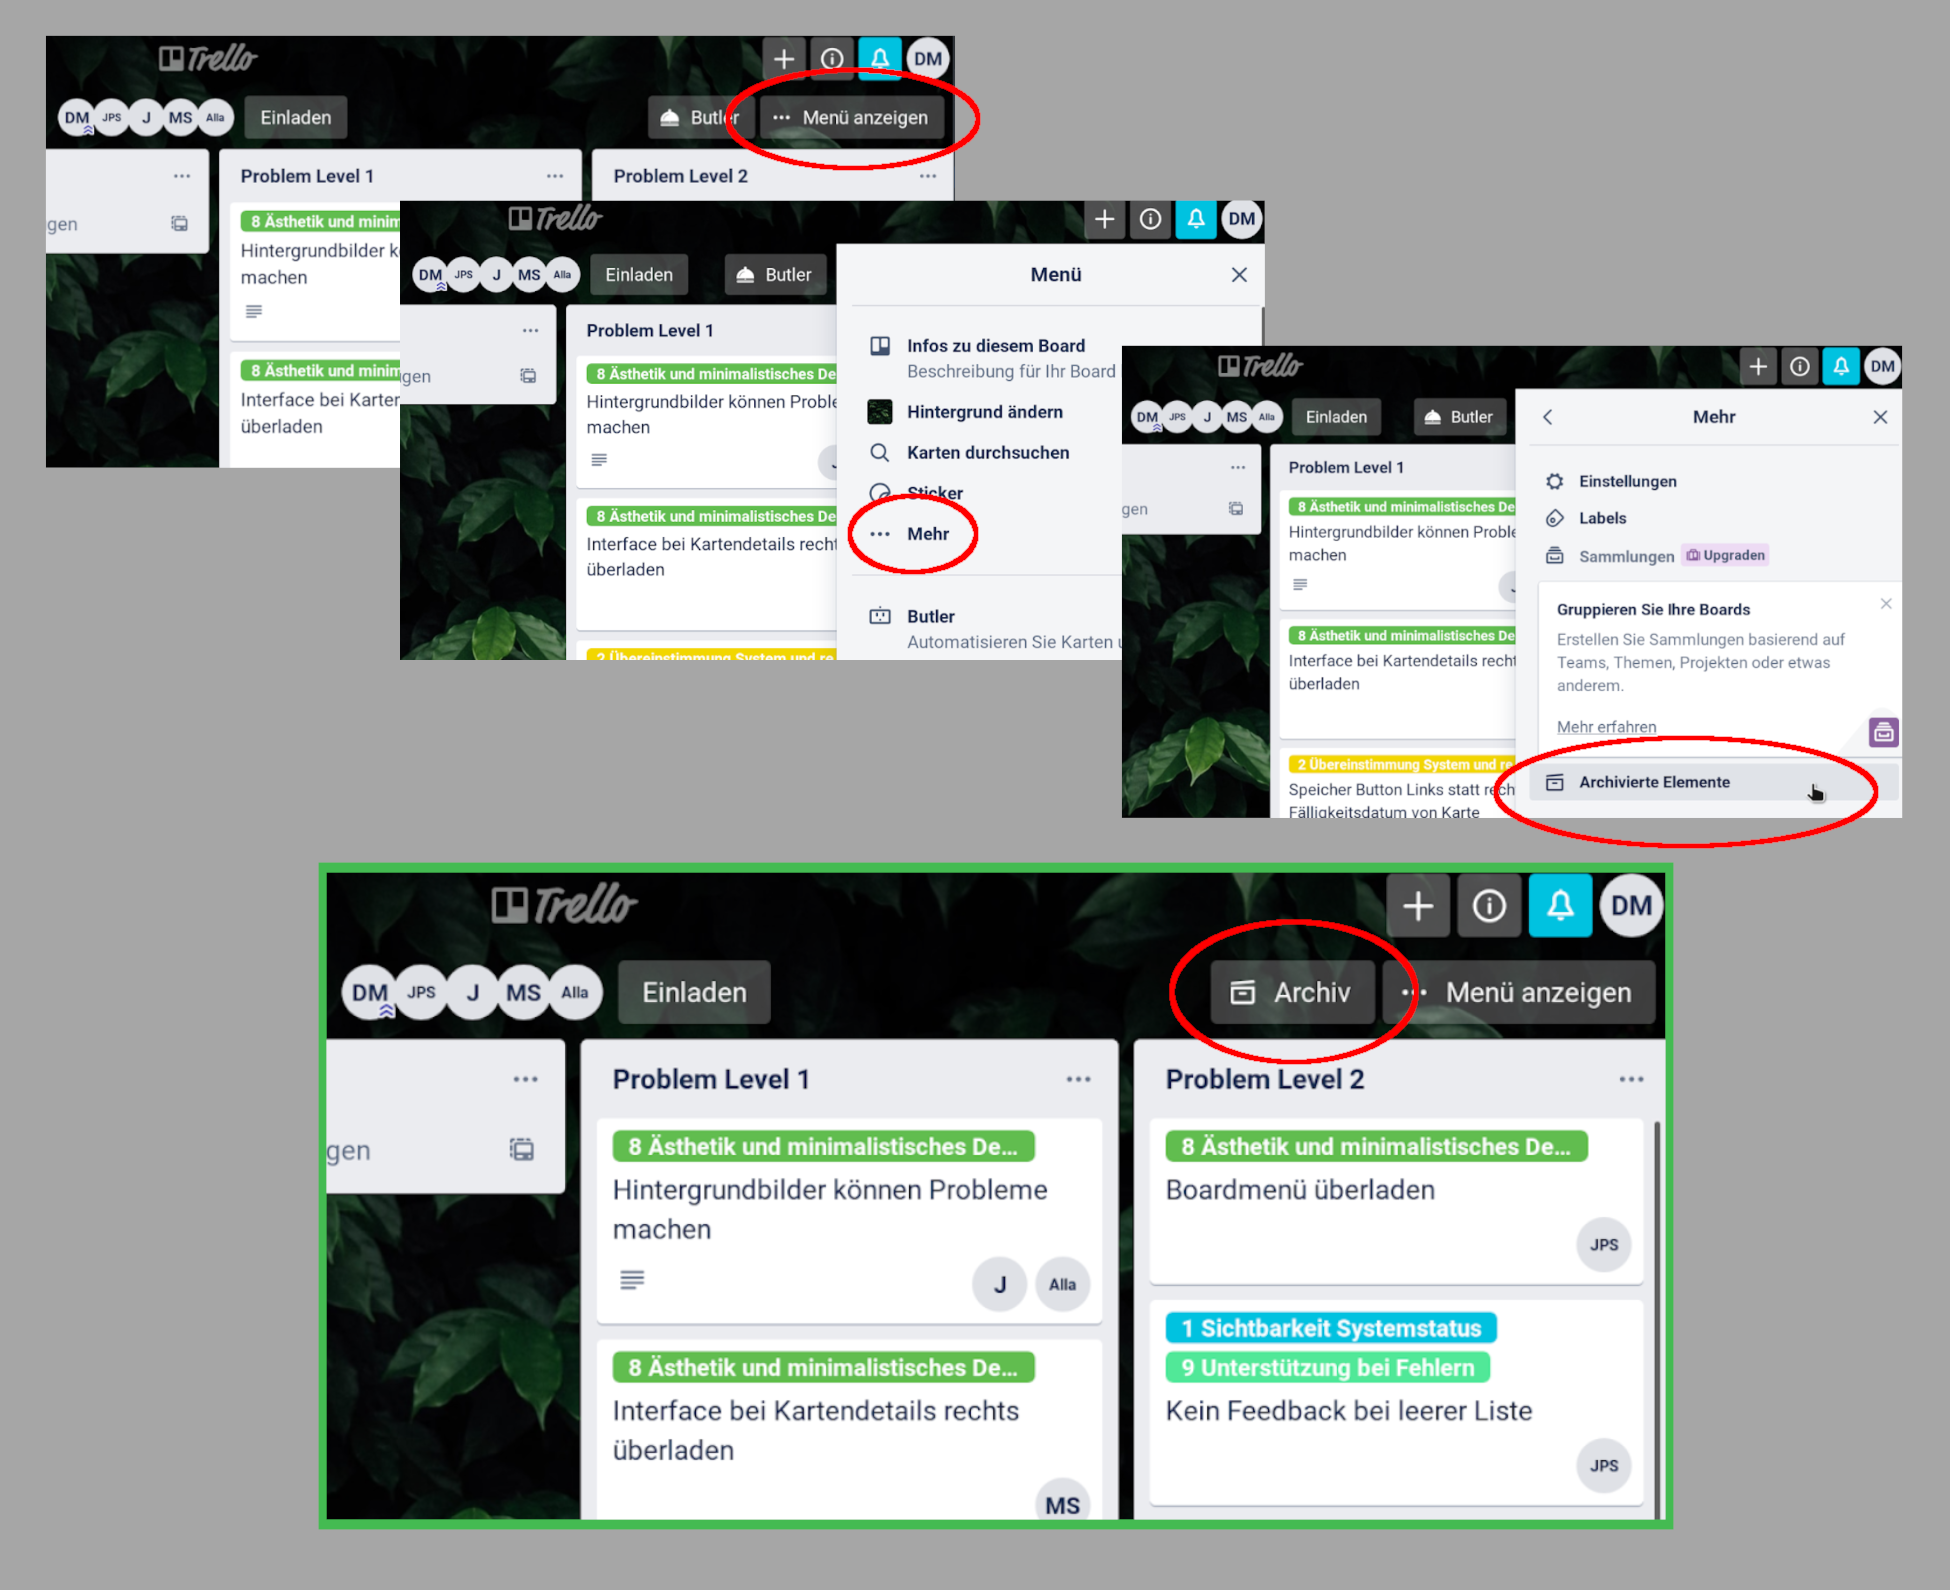
\includegraphics[width=0.9\textwidth]{images/Verbesserungsvorschlaege/2 Archiv.PNG}
    \centering
    \caption{Problemgrad 2: Eine Möglichkeit zum besseren Finden des Archivs (Problem Nr. 15, oben der aktuelle Weg und unten die überarbeitete Version mit eigenem Button)}
    \label{fig:archiv}
\end{figure}

\begin{figure}[h]
    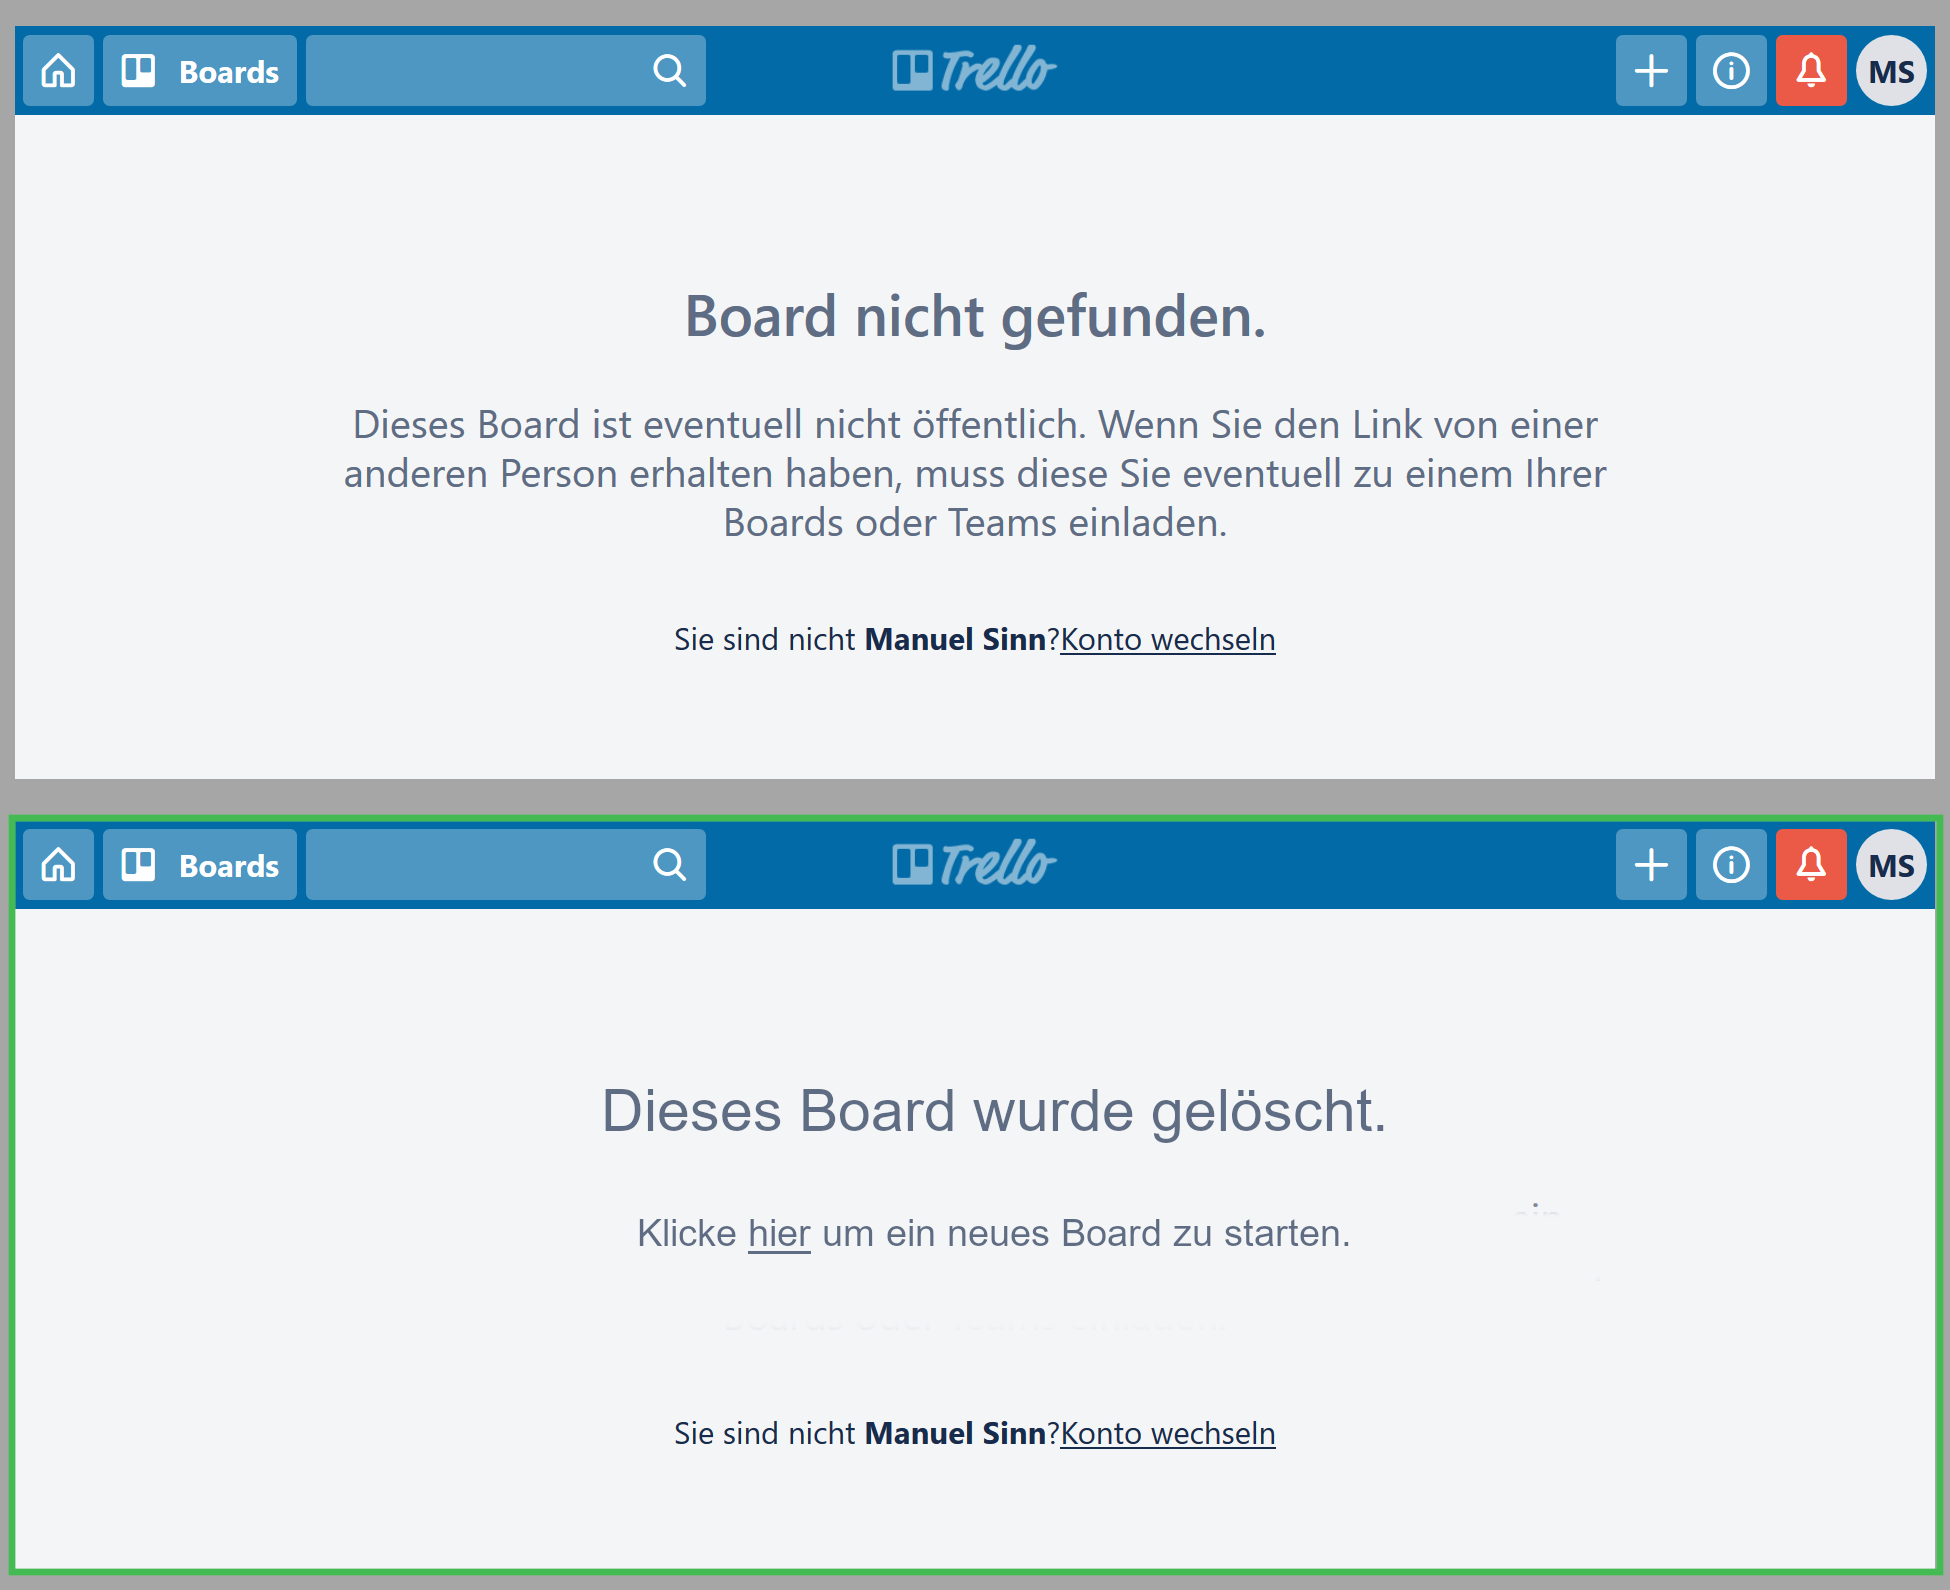
\includegraphics[width=0.7\textwidth]{images/Verbesserungsvorschlaege/3 BoardNichtGefunden.PNG}
    \centering
    \caption{Problemgrad 3: Verbesserung des verwirrenden Feedbacks nach dem endgültigem Löschen eines Boards (Problem Nr. 20, unten die überarbeitete Version)}
    \label{fig:feedback}
\end{figure}

\begin{figure}[h]   
    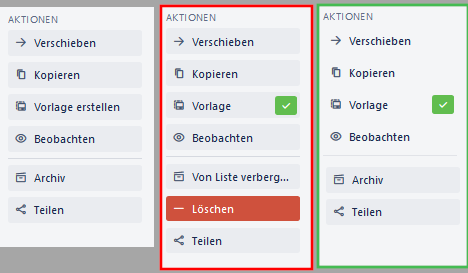
\includegraphics[width=0.6\textwidth]{images/Verbesserungsvorschlaege/4 VorlageErstellen.png}
    \centering
    \caption{Problemgrad 4: Konstanthalten des Menüs statt dem unnötig verwirrendem Verändern bei Wählen der Option 'Vorlage erstellen' (Problem Nr. 9, links die Ausgangssituation, in der Mitte die aktuelle und rechts die überarbeitete Version)}
    \label{fig:vorlage}
\end{figure}
\FloatBarrier




\subsection{Vebesserungsvorschläge Zenkit}
\FloatBarrier
\begin{figure}[h] 
    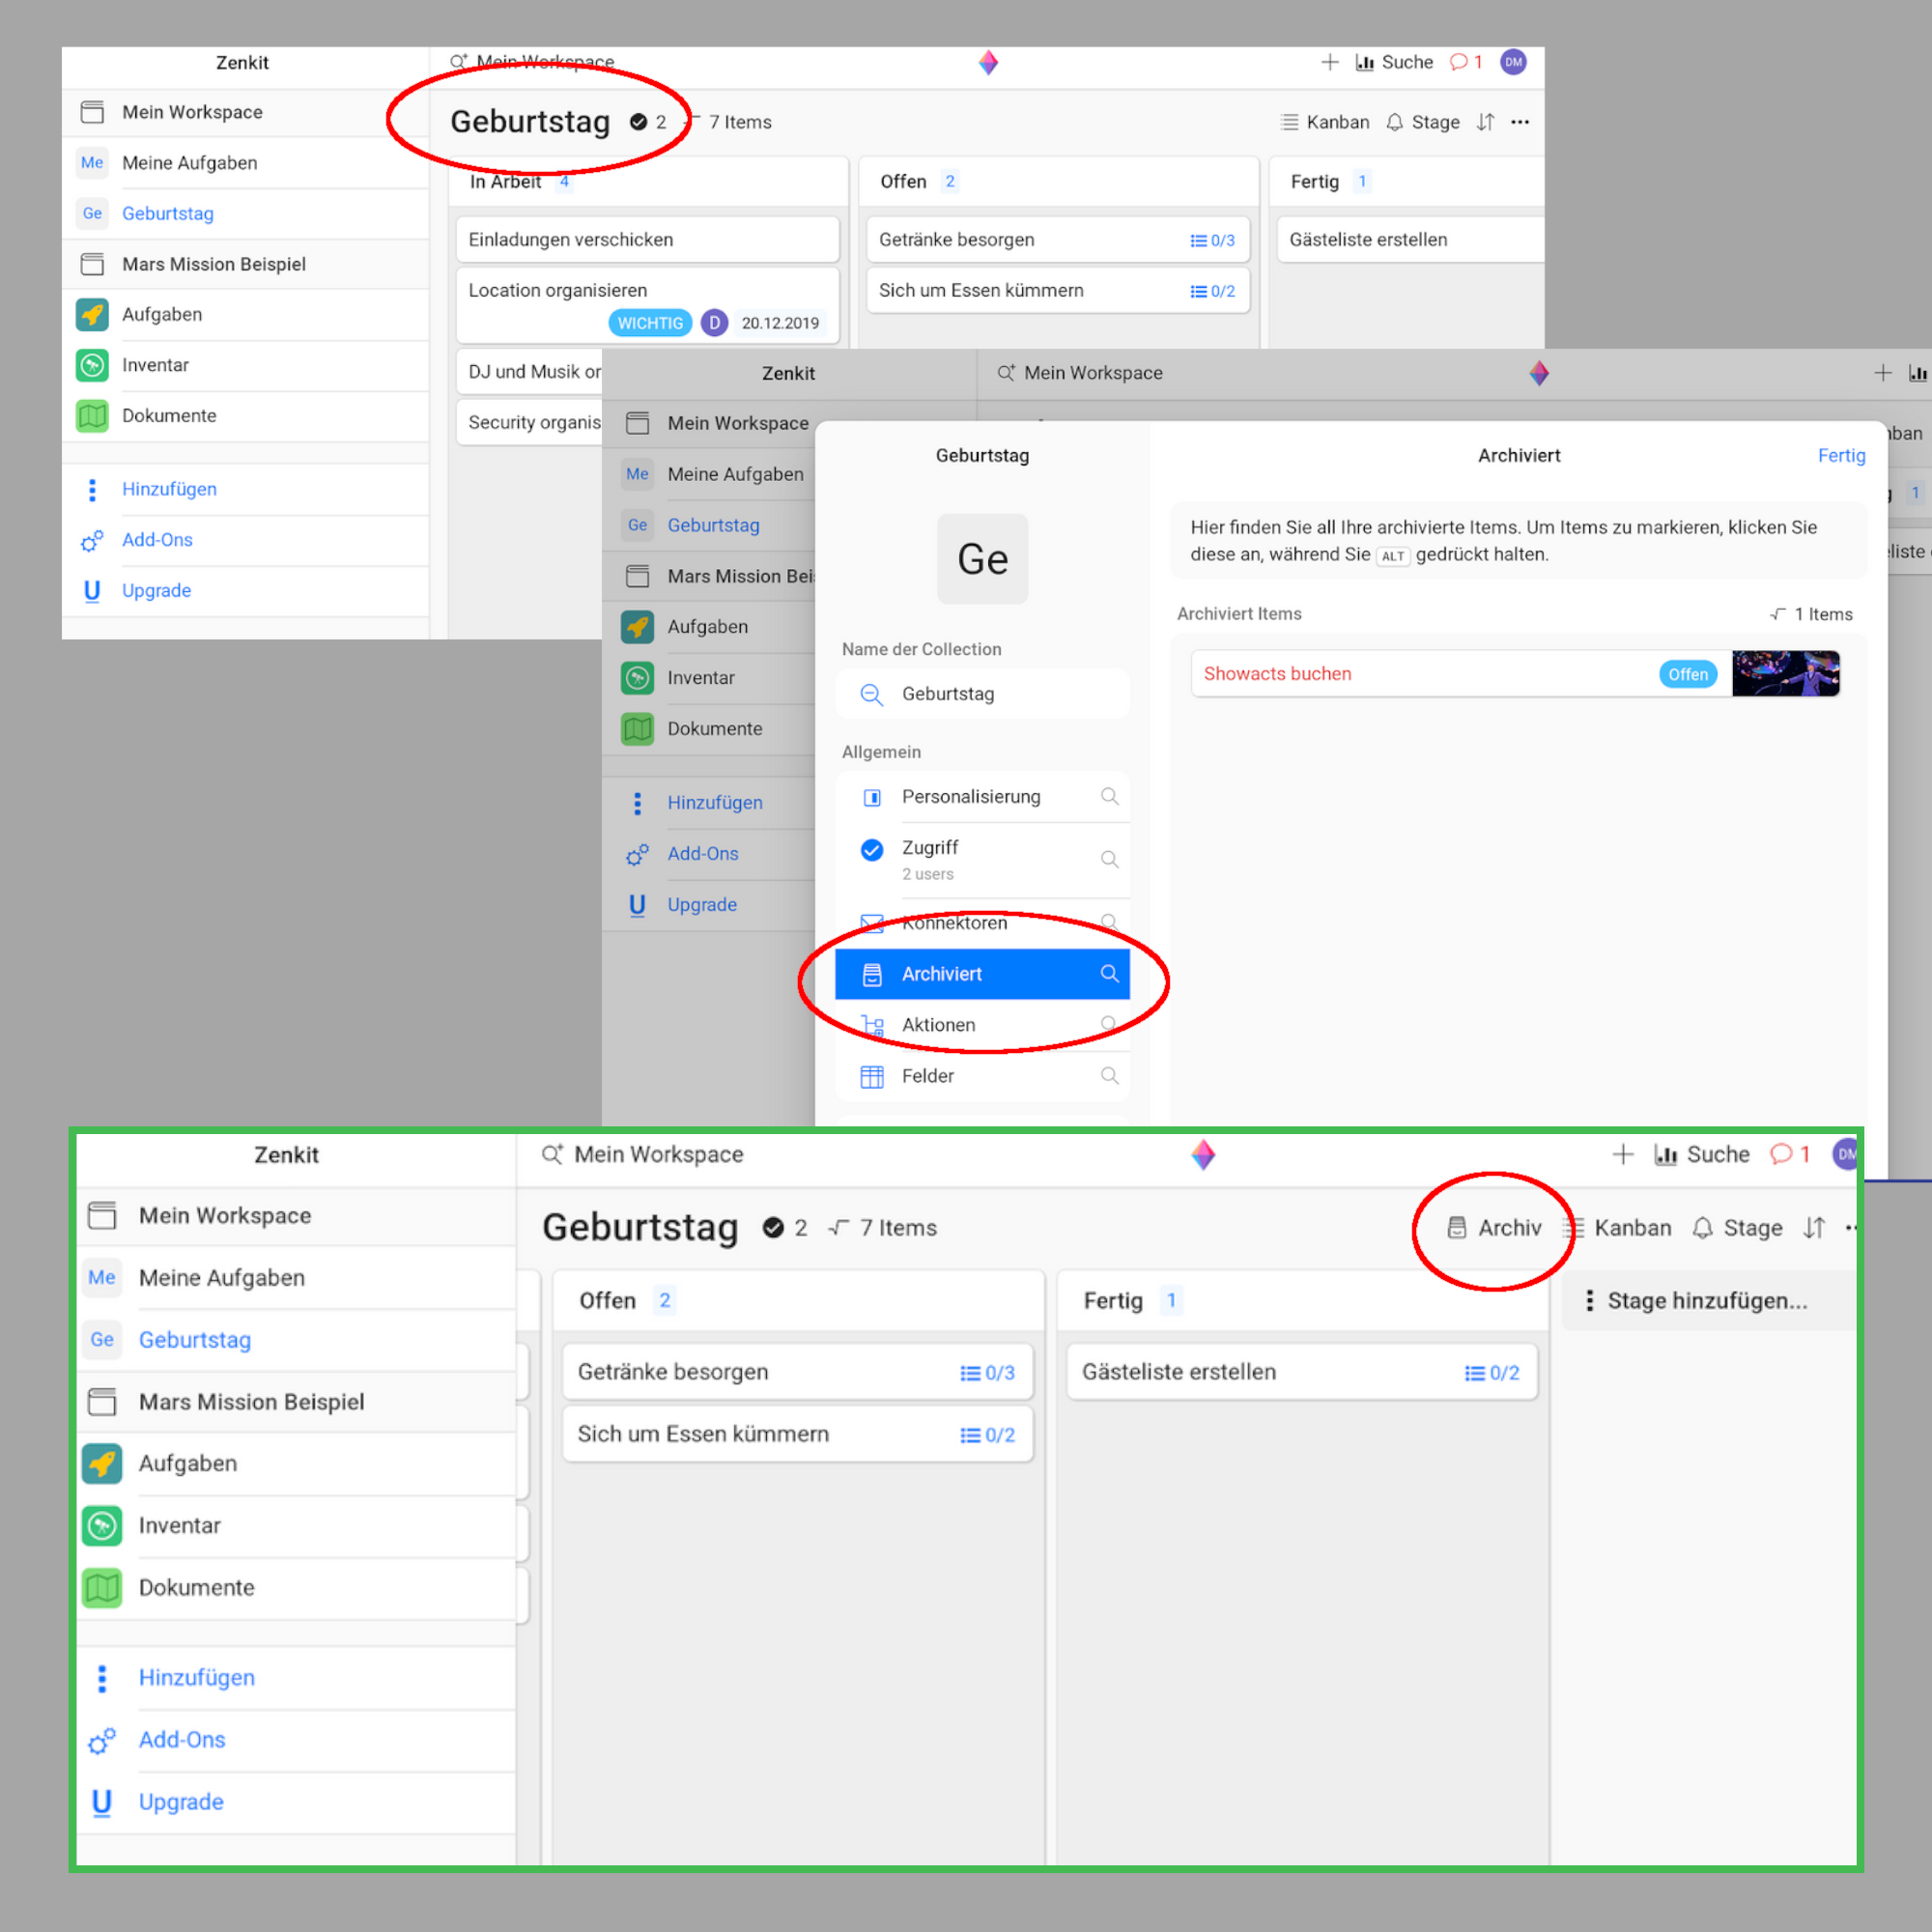
\includegraphics[width=0.6\textwidth]{images/Verbesserungsvorschlaege/zenkitArchiv.png}
    \centering
    \caption{Problemgrad 3, Analog zur Lösung bei Trello, eine Möglichkeit zum besseren Finden des Archivs (Problem Nr. 19, oben der aktuelle Weg und unten die überarbeitete Version mit eigenem Button)}
    \label{fig:zenkitarchiv}
\end{figure}

\begin{figure}[h]   
    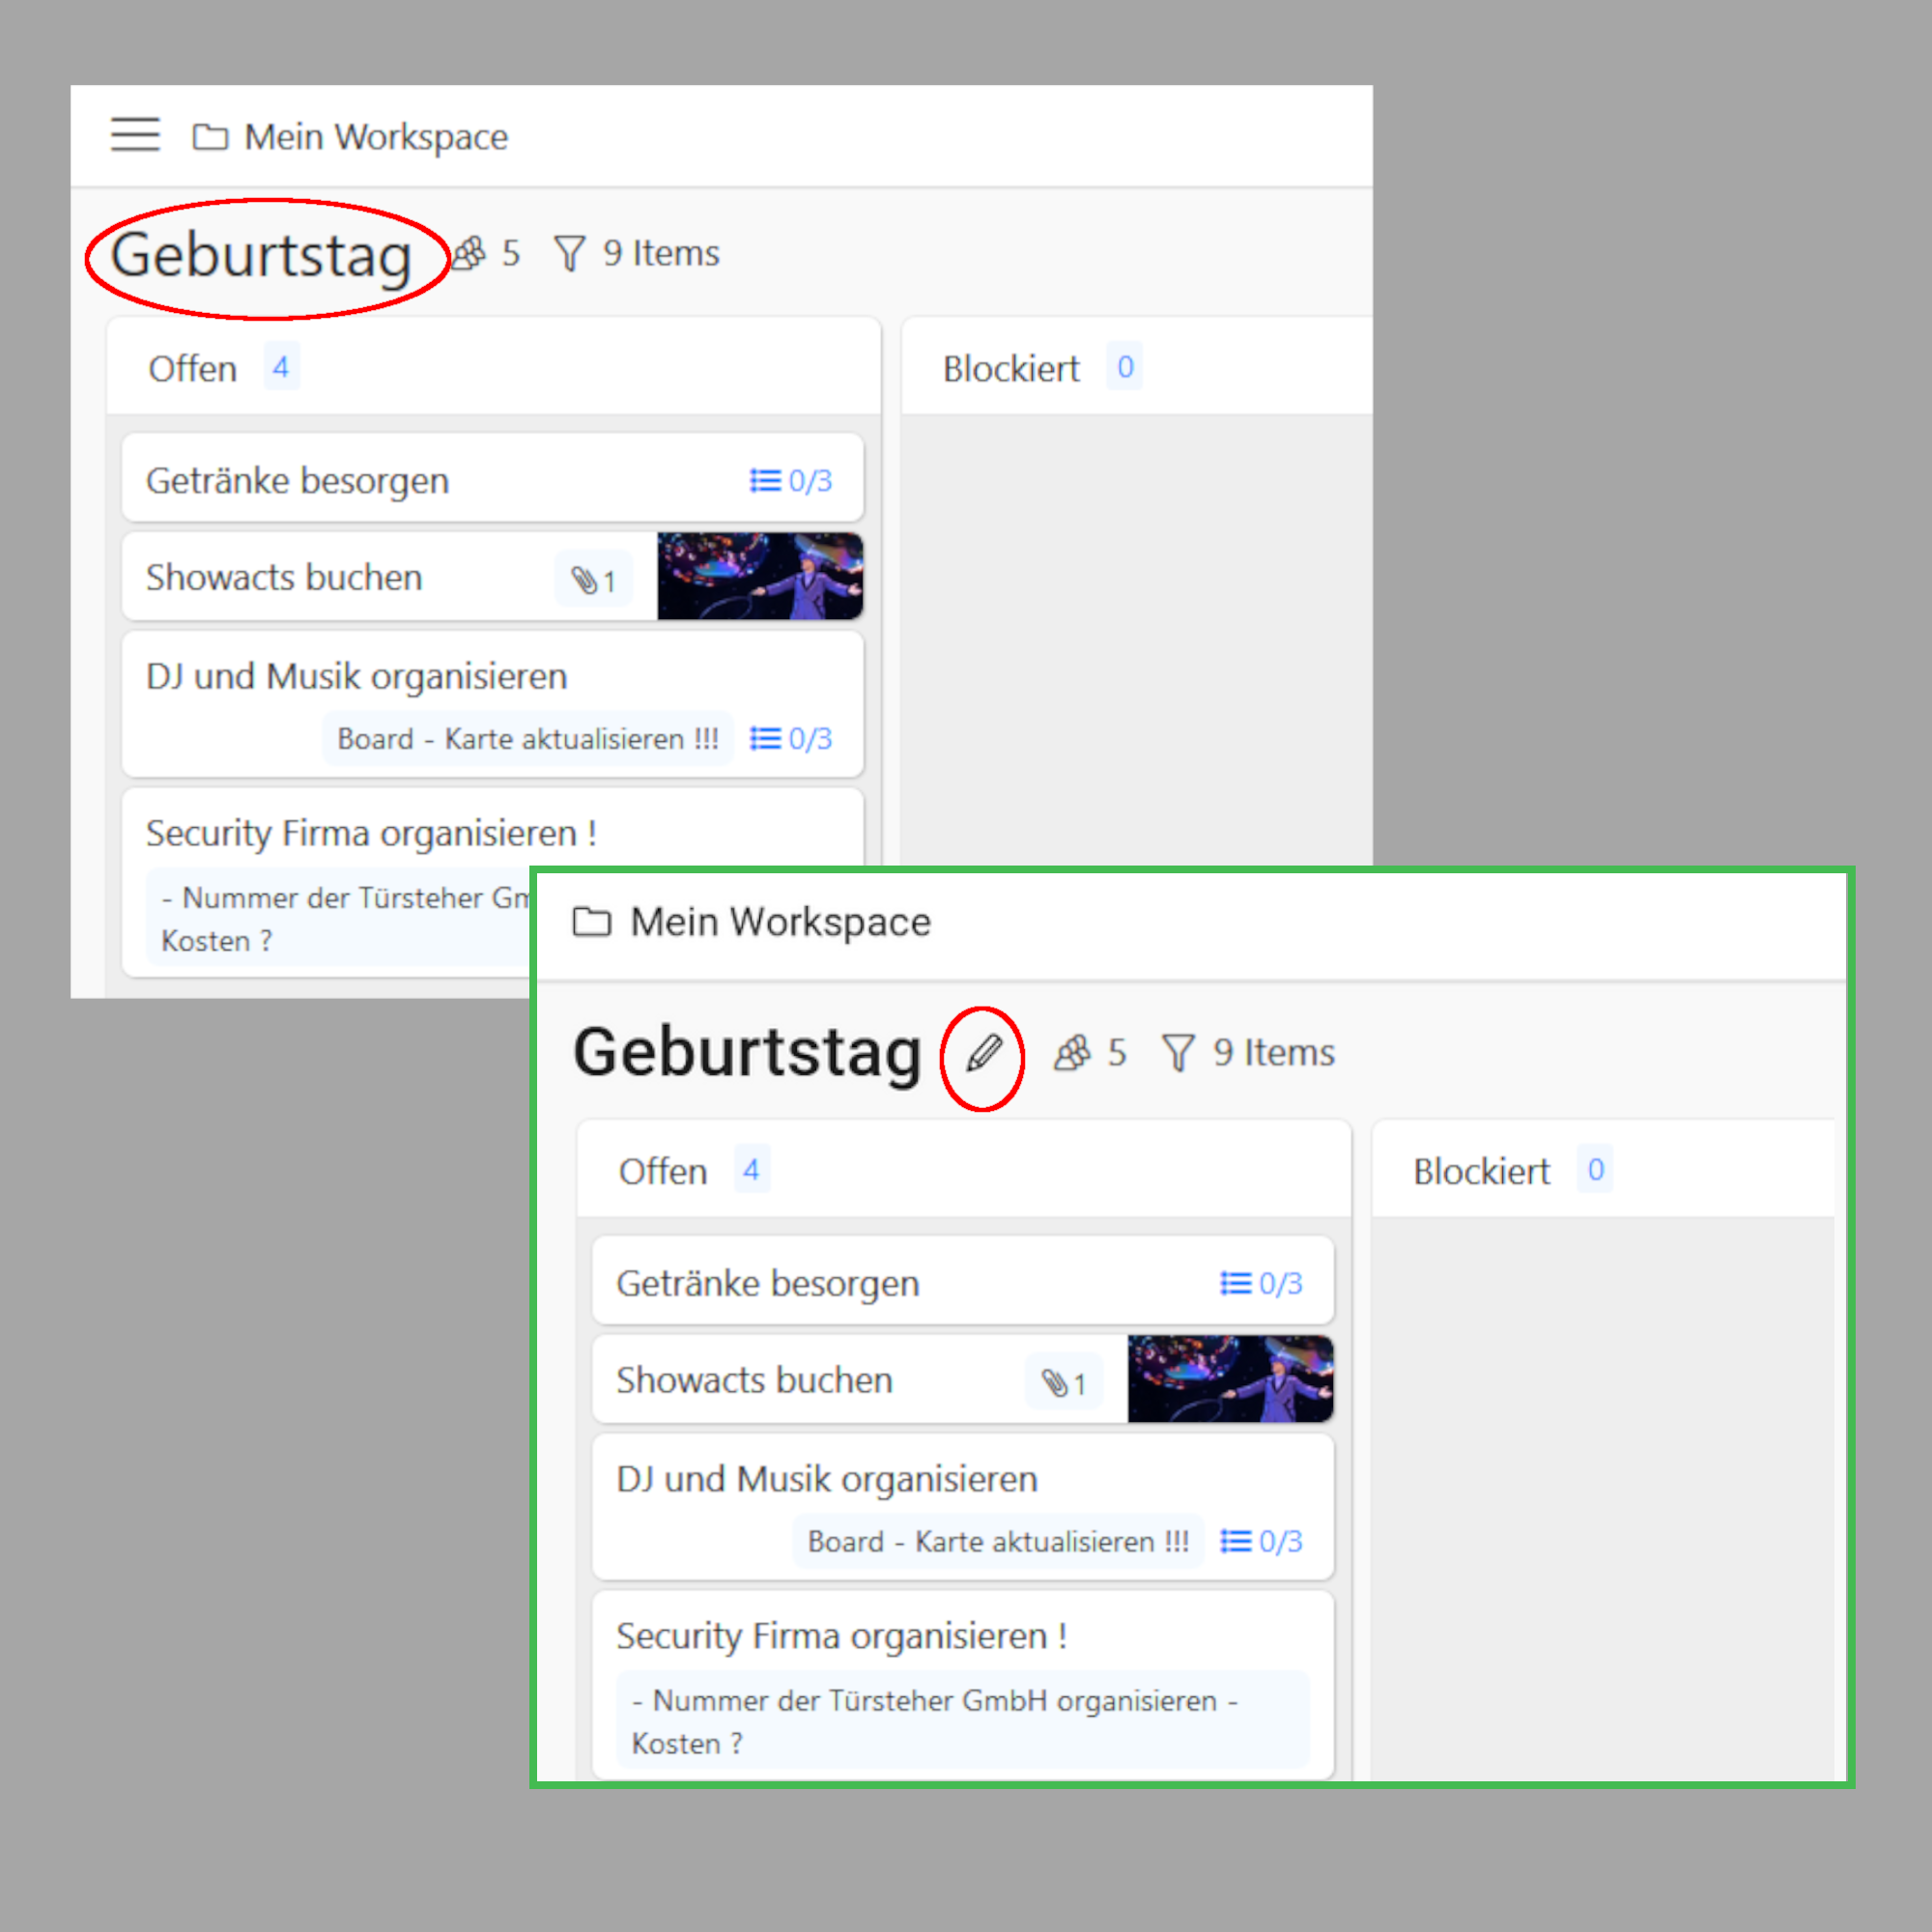
\includegraphics[width=0.6\textwidth]{images/Verbesserungsvorschlaege/ZenkitButton.png}
    \centering
    \caption{Problemgrad 3, Überarbeitung eines für Zenkit typischen Problems, des Versteckens von Bedienelementen (Problem Nr. 20). Der Button für weitere Optionen ist im Namen der Collection 'versteckt', daher wurde in der überarbeiteten Version unten ein eigener Button zum Aufrufen dieser Einstellungen eingefügt.}
    \label{fig:zenkitbutton}
\end{figure}

\begin{figure}[h]
    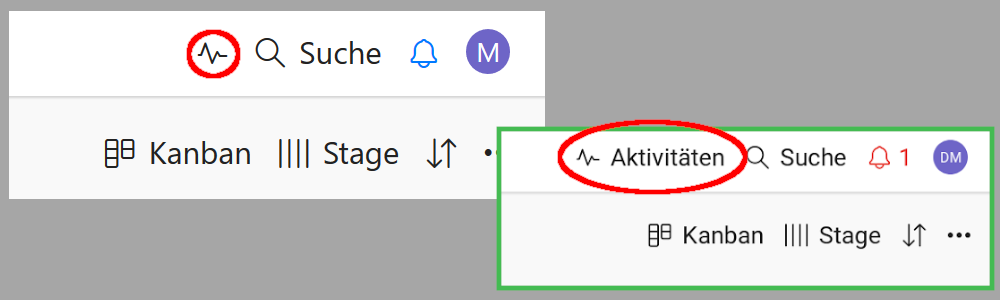
\includegraphics[width=0.6\textwidth]{images/Verbesserungsvorschlaege/zenkitActivities.png}
    \centering
    \caption{Problemgrad 1, Überarbeitung des Aktivitätenbuttons, da dieser schwer aufzufinden und interpretieren war (Problem Nr. 20). Unten die überarbeitete Version mit klarer Benennung.}
    \label{fig:zenkitaktivit}
\end{figure}

\begin{figure}[h]   
    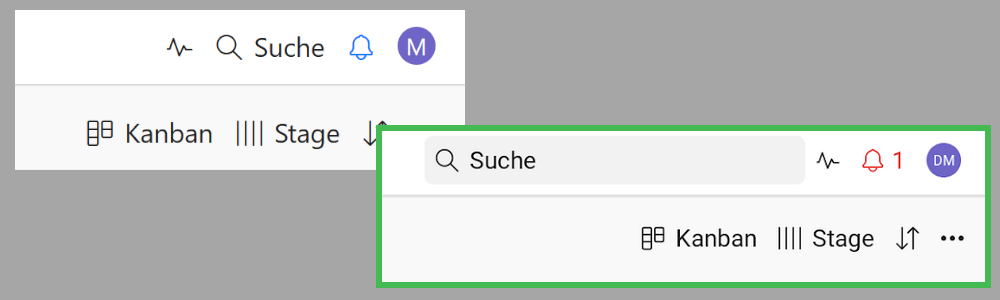
\includegraphics[width=0.6\textwidth]{images/Verbesserungsvorschlaege/zenkitSuche.png}
    \centering
    \caption{Problemgrad 1, Überarbeitung des Suchfeldes, welches, ähnlich wie der Aktivitätenbutton, nicht präsent genug erschien (Problem Nr. 16).}
    \label{fig:zenkitsuche}
\end{figure}

\FloatBarrier